% Fig. 9 -- Ablation and fusion-rule control (single column, 3.5 in).
% Bars = F1 (positive class = fabricated); annotation = missed fabricated alerts out of 63. No variant produced a false positive.
% Numbers: paper/results.md section 2.
% Compile with pdfLaTeX (Overleaf default). Output: fig09_ablation.pdf
\documentclass[border=3pt]{standalone}
\usepackage[T1]{fontenc}
\usepackage{newtxtext,newtxmath}
\usepackage{tikz}
\usepackage{pgfplots}
\pgfplotsset{compat=1.17}

\definecolor{acc}{RGB}{31,78,121}

\begin{document}
\footnotesize
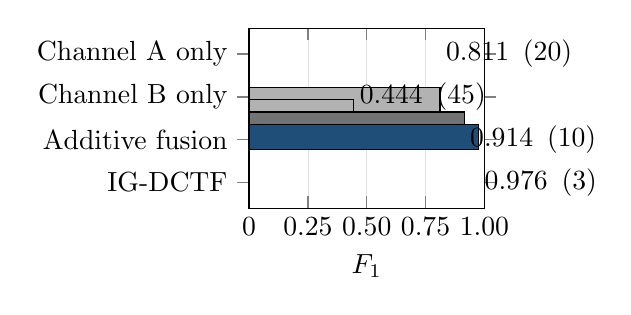
\begin{tikzpicture}
\begin{axis}[
    width=130pt, height=110pt,
    xbar, bar width=9pt,
    xmin=0, xmax=1.0, ymin=-0.6, ymax=3.6,
    xtick={0,0.25,0.5,0.75,1.0},
    xticklabels={0,0.25,0.50,0.75,1.00},
    xlabel={$F_1$},
    ytick={0,1,2,3},
    yticklabels={Channel A only,Channel B only,Additive fusion,IG-DCTF},
    y dir=reverse,
    xmajorgrids, grid style={black!12,line width=0.3pt},
    axis line style={line width=0.5pt}, tick style={line width=0.5pt},
    clip=false,
]
  \addplot[xbar,fill=black!30,draw=black,line width=0.4pt] coordinates {(0.8113,0)};
  \addplot[xbar,fill=black!30,draw=black,line width=0.4pt] coordinates {(0.4444,1)};
  \addplot[xbar,fill=black!55,draw=black,line width=0.4pt] coordinates {(0.9138,2)};
  \addplot[xbar,fill=acc,     draw=black,line width=0.4pt] coordinates {(0.9756,3)};

  % value and miss-count annotations to the right of each bar
  \node[anchor=west,inner sep=2pt] at (axis cs:0.8113,0) {0.811 \,(20)};
  \node[anchor=west,inner sep=2pt] at (axis cs:0.4444,1) {0.444 \,(45)};
  \node[anchor=west,inner sep=2pt] at (axis cs:0.9138,2) {0.914 \,(10)};
  \node[anchor=west,inner sep=2pt] at (axis cs:0.9756,3) {0.976 \,(3)};
\end{axis}
\end{tikzpicture}
\end{document}
